\begin{savequote}[90mm] 
Software is a great combination between artistry and engineering. \qauthor{Bill Gates} 
\end{savequote}

\chapter{Architecture \label{chap:architecture}}

This chapter describes the architecture on which the software is build and how its influence on the results. Figure \ref{fig:architecture} illustrates using course-grained blocks the architecture. The arrows illustrate the data-flow through the system. 

\begin{figure}[ht!]
\centering
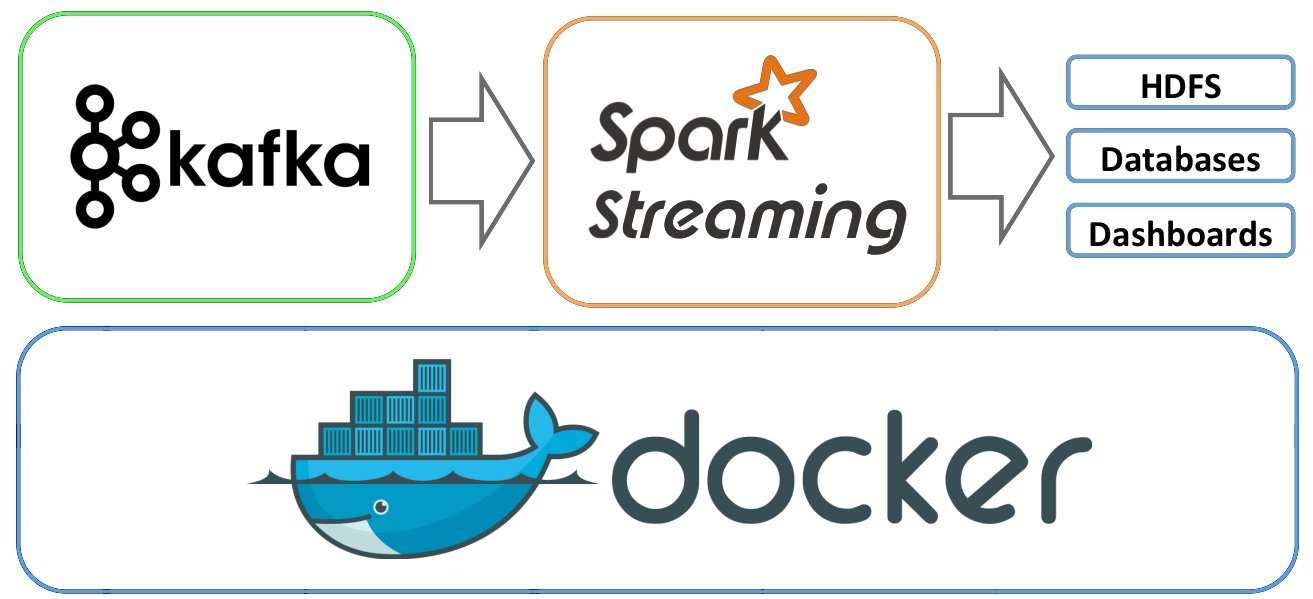
\includegraphics[width=\textwidth]{figures/architecture.jpg}
\caption{Architecture of the system}
\label{fig:architecture}
\end{figure}

The emphasis of the architecture is on scalability. Meaning that it is simple to increase of decrease the number of worker nodes across a number of different physical machines as the machines are provisioned automatically. Tending to implement or evolved to an `elastic architecture' \cite{9780470887998}, which autonomously adapts its capacity to workload over time \cite{180145}, although the number of nodes is configured systematically to determine its performance for a set number of nodes. The underlying provisioning of the resources is done by Docker as described in section \ref{subsec_docker}. The input data on which the algorithm will perform the computations is kept in an Apache Kafka messaging system, described in section \ref{subsec_kafka}. Finally, the computational framework itself build upon Apache Spark is discussed in Section \ref{subsec_spark}.

\begin{figure}[ht!]
\centering

\includegraphics[width=.6\textwidth]{figures/asf.png}
\caption{Logo Apache Software Foundation}
\label{fig:asf}
\end{figure}

Most of the software on which the architecture is build is part of the Apache Software Foundation\footnote{Apache Software Foundation \url{http://www.apache.org/}}, which is a decentralized community of developers across the world. The software produced is distributed under the terms of the Apache License and is therefore free and open source software. The Apache projects are characterized by a collaborative, consensus-based development process and an open and pragmatic software license. 

\section{Docker \label{subsec_docker}}

Docker is an open-source project that automates the deployment of applications inside software containers\footnote{Docker \url{https://www.docker.com/}}. Docker uses resource isolation features of the Linux kernel to allow independent containers to run within a single Linux instance, avoiding the overhead of starting and maintaining virtual machines. Building on top of facilities provided by the Linux kernel, a Docker container, unlike a virtual machine, does not require or include a separate operating system. Docker also simplifies the creation and operation of task or workload queues and other distributed systems \cite{docker1,docker2}.

\begin{figure}[ht!]
\centering
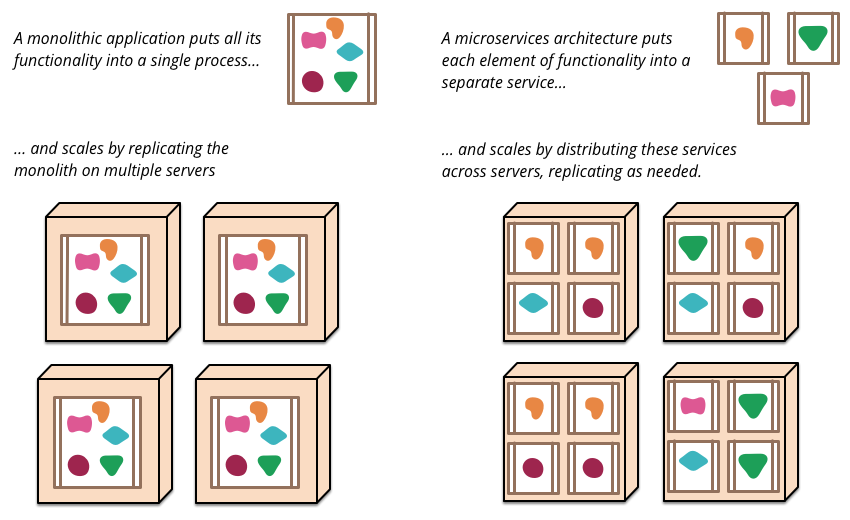
\includegraphics[width=\textwidth]{figures/microservice.png}
\caption{Microservice architecture \cite{microservice} \label{fig:microservice}}
\end{figure}

Docker enables to encapsulate the different applications in lightweight-components which can easily be deployed on top of the docker daemon. This can be a single local docker-daemon or distributed across a pool of physical hosts. This enables deployment of the required components across a group of machines.

The Docker architecture is strongly inspired by the Microservice architecture as depicted in Figure \ref{fig:microservice}. Where every functionality is defined and encapsulated in its own container. Scaling such a system is done by adding or removing service. For example, if there is a computational intensive task scheduled on Spark, more docker-containers can be spawned on the pool of hosts to share the computational workload.

The stack is defined using Docker Compose\footnote{Docker Compose \url{https://www.docker.com/compose/}}, which is the successor of Fig\footnote{Fig \url{http://www.fig.sh/}}. Docker Compose is a tool for defining multi-container applications in a single file. The application with all the dependant containers will be booted using a single command which does everything that needs to be done to get it running.

At this moment Docker is used on a single machine, but can transparently scale to multiple host to create a clustering using Docker Swarm\footnote{Docker Swarm \url{https://docs.docker.com/swarm/}}. 


\section{Apache Spark \label{subsec_spark}}

Apache Spark\footnote{Apache Spark \url{http://spark.apache.org/}} is a computational platform which is designed to be distributed, fast and general purpose. It is an extension on the popular MapReduce model \cite{Dean:2008:MSD:1327452.1327492} and more efficient when it comes to iterative algorithms as it is able to performs in-memory computations \cite{Xin:2013:SSR:2463676.2465288}. Figure \ref{fig:sparkstack} illustrates the Apache Spark is running on top of Docker, but can also run standalone. Spark also includes libraries which specialize in special operation such as machine learning or graph-processing.

\begin{figure}[ht!]
\centering
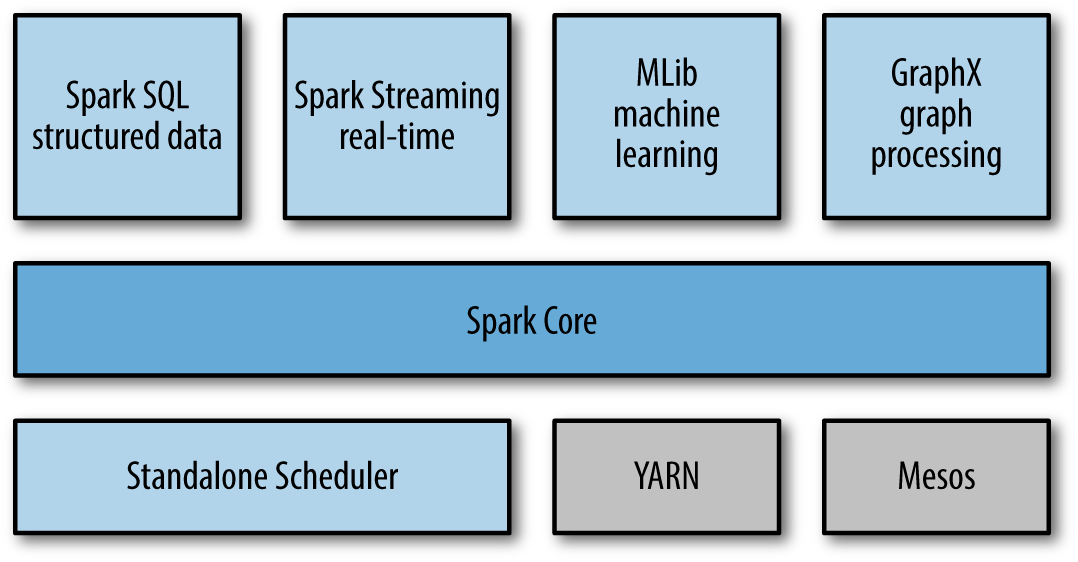
\includegraphics[width=.9\textwidth]{figures/sparkstack.png}
\caption{Apache Spark stack \label{fig:sparkstack}}
\end{figure}

The computational model that Spark follows, consists generally of the following steps:

\begin{description}
  \item[Input-data] Spark is able to fetch the input-data from a variety of sources, including Hadoop Distributed File System, Amazon S3, Apache Flume, Apache Kafka, Apache HBase or any other Hadoop data source.
  \item[Transform] Transformations are defined based on the input data-set. Transformations can be for example, mapping the data to another format, joining different datasets or sorting the data into a specific order.
  \item[Aggregate] After the distributed transform of the data, everything is aggregated and loaded into the driver's local memory or is written to a persistent storage like HDFS.
\end{description}

Apache Spark works with Resilient Distributed Datasets (RDD), which is a read-only, partitioned collection of records. Each transformation within Spark uses a RDD as input and transforms the data into a new RDD. 

Apache Spark will only write to the file-system in a number of situations:
\begin{description}
    \item[Checkpoint] When setting a checkpoint on which it can recover from when data is lost because one or more machines in the clusters are unresponsive as result from a crash or network failure.
    \item[Memory] Every worker works with a subset of the RDD. When the subset grows in such a way that is does not fit in the memory anymore, the data will spill to disk.
    \item[Shuffle] When data needs to be shared across different worker-nodes a shuffle will occur. By designing and implementing an algorithm, these actions should be avoided or kept at an absolute minimum.
\end{description}

An important concept which needs to be taken into account is the number of partitions of a RDD. This is initially set by the source of the RDD. For example, for a \texttt{HadoopRDD} data-source which requests data blocks (64MB by default) from a Hadoop Distributed File System (HDFS), the number of spark-paritions set in park is equal to the number blocks \cite{Dean:2008:MSD:1327452.1327492}. This is a convenient way of managing the number of partitions as the number of partitions grows with the volume of the data. In the case of \texttt{KafkaRDD} which reads from Kafka`s distributed commit log, this is defined by the number of Kafka-partitions in the Kafka-cluster.

It is important to be aware of the number of partitions as it controls the parallelism of the submitted Spark Job. The number of partitions caps the number of tasks which can be executed in parallel. For example, if the RDD has only a single partition, there will be no parallel execution at all.

Spark recommends two or three partitions per CPU core in the cluster\footnote{Apache Spark: Level of Parallelism\url{http://spark.apache.org/docs/latest/tuning.html\#level-of-parallelism}}. This value is heuristically determined and in practice this values needs to be tunes to obtain optimal performance as it differs per type of task.

The Spark Streaming library\footnote{Spark Streaming \url{http://spark.apache.org/streaming/}} introduced in version 1.2 of Apache Spark makes it easy to build scalable fault-tolerant streaming applications. Spark Streaming uses micro-batch semantics, as illustrated in Figure \ref{fig:streaming}.

\begin{figure}[ht!]
\centering
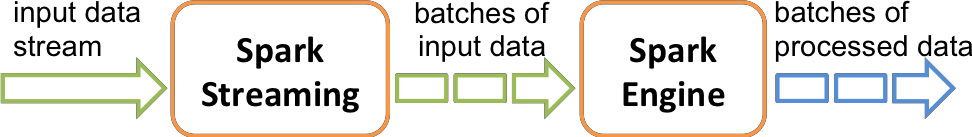
\includegraphics[width=.9\textwidth]{figures/flow.png}
\caption{Spark streaming \label{fig:streaming}}
\end{figure}

By defining a window, for example, for example by a unit of time or per a fixed number of waiting messages. Each time the requirement is full-filled, a new job will be dispatched with as input the window. This streaming concept is particularly well suited using Apache Spark as the data-source.

\section{Apache Kafka \label{subsec_kafka}}

Apache Kafka\footnote{Apache Kafka \url{http://kafka.apache.org/}} provides functionality of a messaging queue in a distributed, partitioned and replicated messaging fashion. Figure \ref{fig:kafka} illustrates the role of Kafka. First, the terminology will be established, which is analogously to message queue's in general:

\begin{description}
    \item[Broker] is a process running on a machine which form together the Kafka cluster. 
    \item[Producer] is a process which publishes messages to the Kafka cluster.
    \item[Consumer] is a process that is subscribed to topics and reads the feed of published messages.
    \item[Topics] is a category identified by a string on which the messages are collected. Each producer and consumer can subscribe to one or more topics on which is writes or reads messages.
    \item[Partition] Each topic is divided into a set of partitions to distribute the topic across a set of different machines.
\end{description}

Producers are in the role of pushing messages into the log and the consumers read the log as messages are appended to the topics which are distributed across multiple machines to split the workload and volume of the data across a number of machines. The high-level topology of an Apache Kafka is given in Figure \ref{fig:kafka}, where three producers which publish messages to the cluster and the three consumers which receive the messages on the topics they are subscribed to.

\begin{figure}[ht!]
\centering
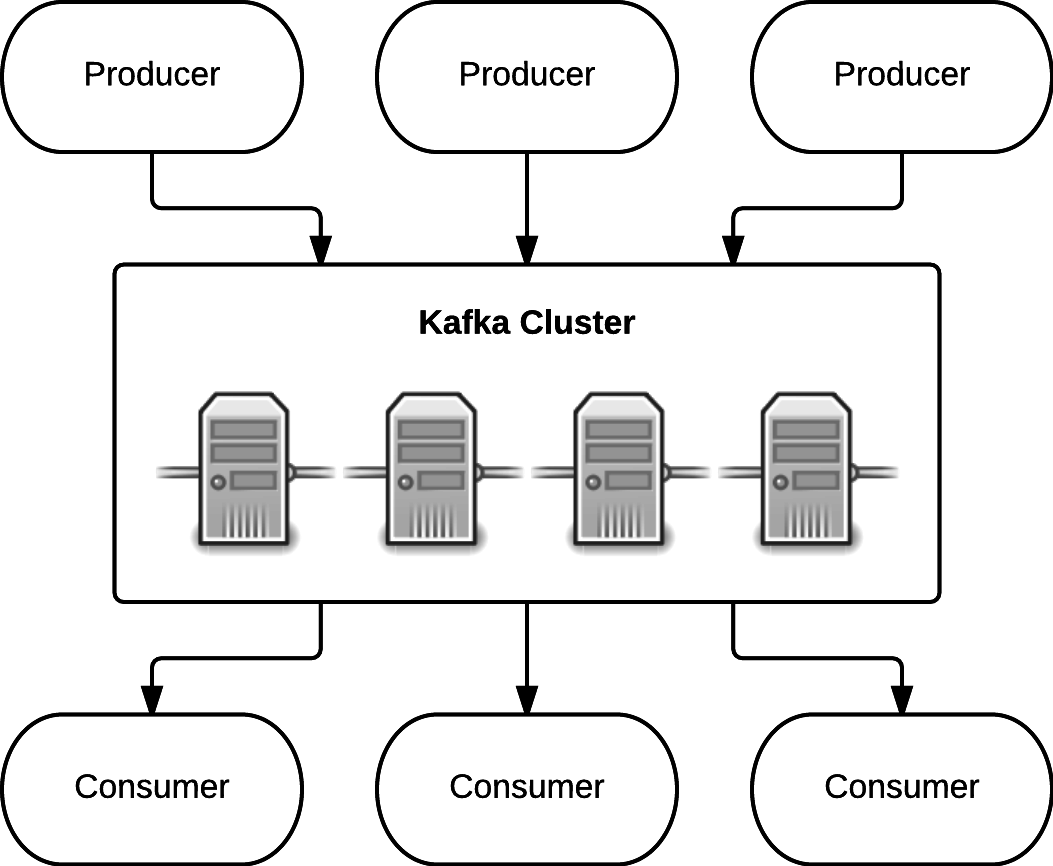
\includegraphics[width=.7\textwidth]{figures/kafka.png}
\caption{Apache Kafka high-level topology. \label{fig:kafka}}
\end{figure}

Apache Kafka is implemented as a distributed commit log, an immutable sequence of messages that is appended as new messages arrive, as illustrated in Figure \ref{fig:kafkalog}. Each messages in the partitions are each assigned a sequential id number called the offset that uniquely identifies each message within the partition. They allow the log to scale beyond a size that will fit on a single server. By default the partitioning is done in a round-robin fashion, but a partitioning algorithm can be implemented to enhance data-locality. 

\begin{figure}[ht!]
\centering
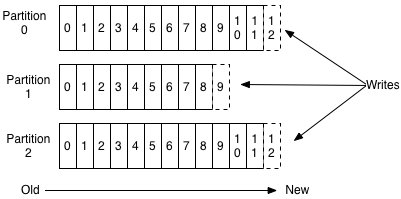
\includegraphics[width=.9\textwidth]{figures/kafkalog.jpg}
\caption{Anatomy of a topic, implemented as a distributed commit log\label{fig:kafkalog}.}
\end{figure}

The performance is effectively constant with respect to data size, so retaining lots of data is not a problem respecting the limitation of fitting a single partition on a single broker. Each partition can be replicated across a configurable number of brokers to ensure fault tolerance and availability of the Kafka cluster.

Apache Kafka allows producers to write arrays of bytes as a record. This means that serializing and deserializing the Scala data-structures has to be done by the programmer. This is done is done in an easy and fast way using the Pickling\footnote{Scala Pickling \url{https://github.com/scala/pickling}} library. 

\section{Apache ZooKeeper \label{subsec_ZooKeeper}}

ZooKeeper\footnote{Apache ZooKeeper \url{https://zookeeper.apache.org/}} is a highly-available coordination service for maintaining configuration, naming, distributed synchronization and providing group services \cite{Hunt:2010}. All of these kinds of services are used in some form or another by distributed applications, including Apache Kafka and Apache Spark. Because of the difficulty of implementing these kinds of distributed services, applications initially usually skimp on them, which make them brittle in the presence of change and difficult to manage. Even when done correctly, different implementations of these services lead to management complexity when the applications are deployed. This is where ZooKeeper steps in.

\begin{figure}[ht!]
\centering
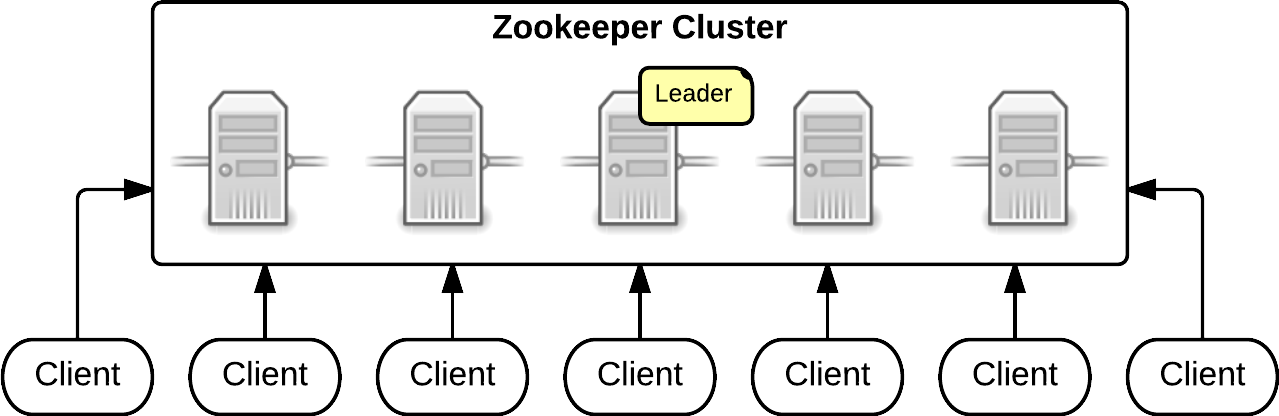
\includegraphics[width=.9\textwidth]{figures/zookeeper.png}
\caption{ZooKeeper topology. \label{fig:ZooKeeper}}
\end{figure}

As depicted in Figure \ref{fig:ZooKeeper}, the ZooKeeper service comprises an ensemble of servers that use replication to achieve high availability and performance. ZooKeeper provides a shared hierarchical name-space which is consistent across all nodes. ZooKeeper runs in memory which ensures high throughput and low-latency.

ZooKeeper replicates the name-space across all nodes using a transaction-log which ensures that all the mutations performed by the majority of the ZooKeeper-instances in the cluster. The operations on ZooKeeper are wait-free and does not uses blocking operations such as locks. This is implemented in the leader-based atomic broadcast
protocol named ZooKeeper Atomic Broadcast (ZAB) \cite{zab} which implements the following guarantees \cite{Hunt:2010}:

\begin{description} 
    \item[Linearizable writes] all requests that update the state of ZooKeeper are serializable and respect precedence.
    \item[FIFO client order] all requests from a given client are executed in the order that they were sent by the client.
\end{description}

As long as a majority of the servers are correct, the ZooKeeper service will be available, with a total of $2f+1$ Zookeeper processes, it is able to tolerate $f$ failures. When the cluster becomes partitioned, from for example a network failure, the partitions with the number of processes smaller than $f$ will become available and falls down to an auto-fencing mode, rendering the service unavailable \cite{0201619180}.

An interesting and useful feature of ZooKeeper are ephemeral nodes. These are nodes in the hierarchical name-space of the ZooKeeper service which will be removed as the process which created them disconnects of becomes unavailable. This enables the ZooKeeper service to only show the list of nodes which are available.

In the software-stack used for the experiment, ZooKeeper is used for:
\begin{description} 
    \item[Apache Kafka] a master is elected for each partition within a topic. This is needed if a partition is replicated, one master is assigned which the slaves will follow, if the master dies a new master gets elected out of the slaves. 
    \item[Apache Spark] Spark allows to have multiple masters of which only one is active. If the master dies, a standby-master can take over and resubmit the job.
\end{description}

\section{Software}

The software will be written on top of the architecture as described above. The software will use the Spark Driver to communicate with the cluster. The way this works is illustrated in Figure \ref{fig:driver}. Instead of submitting a packed program to the cluster, the driver tells the worker nodes where the data is and the transformations are serialized and transferred to the worker nodes.

\begin{figure}[ht!]
\centering
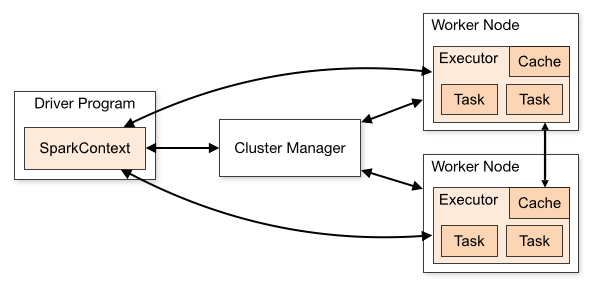
\includegraphics[width=\textwidth]{figures/clusterdriver.png}
\caption{Spark context which sends the job to the worker nodes. \label{fig:driver}}
\end{figure}

The Spark-driver will also be deployed on the server as a Docker container. This will ensure that the driver will run on the same cluster and network communication between cluster and the executors will be minimal.

The software is build using Simple Build Tool\footnote{Simple Build Tool \url{http://www.scala-sbt.org/}} (SBT) which handles the flow of testing, running and packaging. Using the SBT Assembly plugin \footnote{SBT Assembly \url{https://github.com/sbt/sbt-assembly}} a JAR file is generated which contains all the source and the libraries it depends on. By packing specific versions of the dependant libraries into the JAR prevents the need of additional libraries to be available at run-time.

The source of the algorithm is placed in a GIT\footnote{GIT Version Control \url{https://git-scm.com/}} version control system called Github\footnote{Github \url{https://github.com/rug-ds-lab/SparkOutlierDetection}}, which keeps track of changes to the source code. The Github allows the developer to attach hoops to events, such as the push of new code to the repository.

As continuous integration server Travis\footnote{Travis CI \url{https://travis-ci.org/rug-ds-lab/SparkOutlierDetection}} is used to build a new version of the software each time a new push is done to the Github repository. The test-coverage of the software is tracked using Codecov\footnote{Codecov \url{https://codecov.io/github/rug-ds-lab/SparkOutlierDetection}}. Using Codecov the test-coverage is visualized per line of code, and gives suggestions which files require additional test-coverage. 
Codacy\footnote{Codacy \url{https://www.codacy.com/app/fokko/SparkOutlierDetection}} is used to keep track of the quality of code by performing static analysis on the code, each time changes are applied the code is searched for Scala specific code-smells which might incur errors, such as the creation of threads instead of using futures, the use of reserved key-words, high cyclomatic complexity or the use of \texttt{var} instead of the immutable \texttt{val}. 
